\documentclass{beamer}
\usetheme{Warsaw}

\fontfamily{pag}
\usepackage{libertine}
\usepackage{animate} %need the animate.sty file
\renewcommand*\familydefault{\sfdefault}

\setlength{\parskip}{1em}

\setbeamercolor{normal text}{fg=white,bg=black!90}
\setbeamercolor{structure}{fg=white}

\setbeamercolor{alerted text}{fg=red!85!black}

\setbeamercolor{item projected}{use=item,fg=black,bg=item.fg!35}

\setbeamercolor*{palette primary}{use=structure,fg=structure.fg}
\setbeamercolor*{palette secondary}{use=structure,fg=structure.fg!95!black}
\setbeamercolor*{palette tertiary}{use=structure,fg=structure.fg!90!black}
\setbeamercolor*{palette quaternary}{use=structure,fg=structure.fg!95!black,bg=black!80}

\setbeamercolor*{framesubtitle}{fg=white}

\setbeamercolor*{block title}{parent=structure,bg=black!60}
\setbeamercolor*{block body}{fg=black,bg=black!10}
\setbeamercolor*{block title alerted}{parent=alerted text,bg=black!15}
\setbeamercolor*{block title example}{parent=example text,bg=black!15}

\usepackage{grffile} %for underscores in file names
\usepackage{gensymb} % degree
\title{The Science of Brewing:}
\subtitle{How 4 simple ingredients become the best beverage in the world \newline \newline Part 2: Hops}
\date{\footnotesize{\today}}
\author{Nick Waters}
\institute{Department of Microbiology\\
School of Natural Sciences\\
National University of Ireland, Galway}

\begin{document}
\maketitle

\begin{frame}
\frametitle{Ingredients}
\begin{enumerate}
\item Barley
\item Hops
\item Water
\item Yeast
\end{enumerate}
\end{frame}

\begin{frame}
\begin{center}
    \hspace*{-10mm}\includegraphics[width=1.2\textwidth]{./brewing/overview.jpg}
    \end{center}
\end{frame}

\section{Introduction}

\begin{frame}
\frametitle{Disclaimer}
\begin{enumerate}
\item I am not an expert
\end{enumerate}
\end{frame}


% Hops:  what are they?
% - diagram
% - picture of a hop field

\begin{frame}\frametitle{Hops}
\begin{itemize}
\item \textit{Humulus lupulus}
\item flower, cone, strobilus
\end{itemize}
\includegraphics[width=.6\linewidth]{./brewing/hops/Cascadehopsinthesun.jpg}
\hspace{5mm}
\end{frame}


\begin{frame}\frametitle{Hops}
\centering\includegraphics[width=\linewidth]{./brewing/hops/Cross-section-dark.pdf}
\end{frame}

\begin{frame}\frametitle{History of Hop Cultivation}
  \begin{itemize}
  \item Documented cultivation between 736--1079 in Hallertau, Germany
  \item Pepin the Short left hop gardens to Charlemagne in 768
  \item Hopped beer introduced to Britain in 1400
  \item Hops cultivated in England 1524
  \item Hops cultivated in America 1629
  \end{itemize}
  \centering\includegraphics[width=.5\linewidth]{./brewing/hops/bohemia}
\end{frame}

\begin{frame}\frametitle{Modern Cultivation}
  \begin{itemize}
  \item Dioecious: males not used for brewing
  \item Bines trained over strings on trestles
  \item Susceptible to mold and mildew
  \end{itemize}
  \centering  \includegraphics[width=.7\linewidth]{./brewing/hops/Hopfengarten.jpg}
\end{frame}



\section{Why hops?}

\begin{frame}\frametitle{Unhopped beer}
  \begin{columns}
    \begin{column}{0.6\textwidth}
    \begin{itemize}
    \item Yeast never 100\% effective; beer is sweet
    \item Gruit: bitter spice mixure: sweet gale, mugwort, yarrow, ground ivy, horehound, and Calluna heather, juniper berries, ginger, caraway seed, aniseed, nutmeg, cinnamon, etc.
    \item More expensive, more prone to spoilage
    \end{itemize}
  \end{column}
  \begin{column}{0.5\textwidth}
    \begin{center}
      \centering  \includegraphics[width=.7\linewidth]{./brewing/hops/Gruit-Mixture.jpg}
    \end{center}
  \end{column}
  \end{columns}
      \tiny{http://www.gruit.es/en/brewmaster-1a-part/}
\end{frame}

\begin{frame}\frametitle{Hopped beer}
  \begin{columns}
    \begin{column}{0.6\textwidth}
    \begin{itemize}
    \item Cheap
    \item Antibacterial properites
    \item Tasty!
    \end{itemize}
  \end{column}
  \begin{column}{0.5\textwidth}
    \begin{center}
      \centering  \includegraphics[width=\linewidth]{./brewing/hops/Hopfendolde-mit-hopfengarten.jpg}
    \end{center}
  \end{column}
  \end{columns}
\end{frame}

\section{What's in Hops?}


\begin{frame}\frametitle{Hops are:}
  % \begin{itemize}
  % \item alpha acids
  % \item beta acids
  % \item oils
  % \item flavenoids
  % \item other stuff
  % \end{itemize}
\begin{table}[]
\centering
\label{components}
\begin{tabular}{lr}
  \textbf{Components} & \textbf{(\%w/w)} \\
  Cellulose + lignin & 40.0 \textemdash 50.0 \\
  Protein & 15.0 \\
  {\color{green}$\alpha$ acids} & 2.0 \textemdash 17.0  \\
  {\color{green}$\beta$ acids} & 2.0 \textemdash 10.0 \\
  Minerals & 8.0 \\
  Polyphenols and tannins & 3.0 \textemdash 6.0 \\
  Lipids and fatty acids & 1.0 \textemdash 5.0 \\
  {\color{green}Hop oil} & 0.5 \textemdash 3.0 \\
  Monosaccharides & 2.0 \\
  Pectin & 2.0\\
\end{tabular}
\end{table}
\tiny{European Brewery Convention Hops and Hop Products, Manual of Good Practice; Getranke - Fachverlag Hans Carl: Nurnberg, Germany, 1997. Water not shone}
\end{frame}

% \begin{frame}\frametitle{$\alpha$ acids (Humulones)}
%   \centering
%   \animategraphics[autoplay,loop,controls,poster=last,height=3.9cm]{100}{brewing/hops/animations/humulone_}{0}{179}

% \end{frame}


\begin{frame}\frametitle{$\alpha$ acids (Humulones)}
  \includegraphics[width=.85\textwidth]{./brewing/hops/isomerization.jpg}
  \begin{itemize}
  \item Bitter (IBU measuring)
  \item Antimicrobial
  \item ``skunking'': sun + isohumulones $\rightarrow$ free radicals $\rightarrow$ thiols
    \item Good bitterness
  \end{itemize}
\end{frame}


\begin{frame}\frametitle{$\beta$ acids (Lupulones)}
  \includegraphics[width=.5\textwidth]{./brewing/hops/Lupulone-dark.pdf}
  \begin{itemize}
    \item Bad bitterness
  \end{itemize}
\end{frame}

\begin{frame}\frametitle{Essential Oils}
  Myrcene 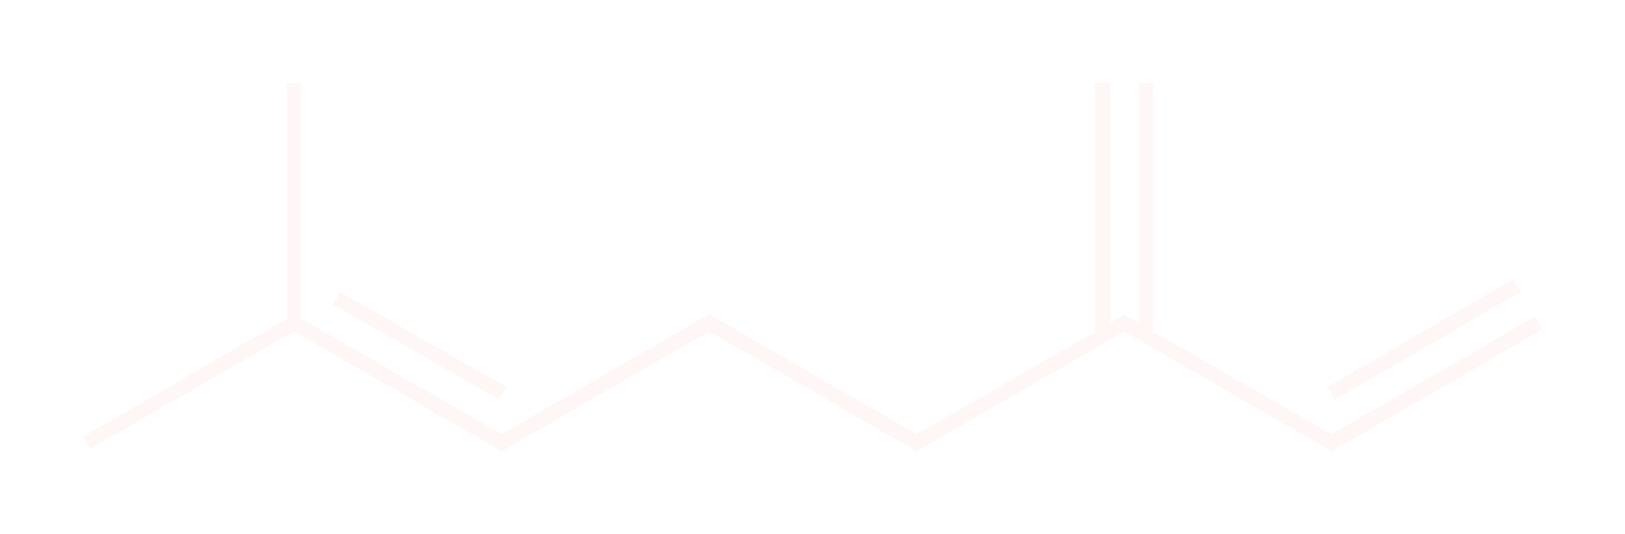
\includegraphics[width=.25\textwidth]{./brewing/hops/Myrcene-dark.pdf}
  \begin{itemize}
  \item Thyme, cannabis, lemmongrass, bay leaf, mango, lavender
  \item Unstable; prone to Diels-Alder reactions
  \end{itemize}
  Humulene \includegraphics[width=.15\textwidth]{./brewing/hops/Humulene-dark.pdf}
  \begin{itemize}
  \item Ginger
  \item
  \end{itemize}
\end{frame}





\section{The Pursuit of Hoppiness}
% measuring IBUs
% ibu by style chart
% chart of heat stability
% bittering hops 30 - 90
% flavour hops 10 - 30
% aroma hops 0-10
% dry hopping +

\section{Hop Varieties}

% varieties: Noble or New world
% German/Czeck Noble
% Engligh Noble







% \begin{frame}
%   \frametitle{Sources}
%   \begin{enumerate}
%   \item http://howtobrew.com/book/section-3/how-the-mash-works/mashing-defined
%   \item https://www.britannica.com/plant/barley-cereal
%   \item https://www.slideshare.net/kourtney-kathryn/advanced-foods-presentation-beer
%   \item https://www.integrowmalt.com/about-integrow/malting-barley-storage.html
%   \item http://www.morebeer.com/brewingtechniques/bmg/schwarz.html
%   \item http://wynwoodbrewing.com/wp-content/uploads/2013/08/WBcoBrewingProcess-4.jpg
%   \end{enumerate}
%   \end{frame}

\end{document}
